\ifbook {
  \mysubsection{Remarque préliminaires}
  \paragraph{} \textit{Le champ d'expertise de l'auteur de ce document est Java/JEE, et plus spécifiquement,
  les produits JBoss. Cet état de fait n'est pas sans conséquence sur le contenu du cours, qui
  s'appuye souvent des composants logicielle spécifique à Java.}

  \paragraph{} \textit{Ainsi, bien que la plupart des concepts évoqués dans cette partie se retrouvent
  généralement, sous une forme ou une autre, dans d'autres univers technologique, certains seront
  néanmoins parfois relativement spécifique à l'univers Java ou au monde JBoss.}

  \paragraph{} \textit{Dans la mesure du possible, lorsque ces cas seront évoqués, leur spécifités sera
  soulignés. Le lecteur devra tout de même rester vigilant...}

}

\mysubsection{Conteneur d'exécution virtuelle}

\ifbook {
  \mysubsubsection{Difficultés des applications natives}

  \paragraph{} Reprenons là où nous avons arrêté, dans le section précédente, la description d'un
  serveur. Nous avions donc une machine physique ou virtuelle dont les resources (mémoire,
  entrées/sorties, processeurs) sont partagé par l'intermédiaire du système d'exploitation, qui joue
  le rôle d'arbitre entre les différentes applications.

  \paragraph{} Si ce modèle fonctionne très bien, et de nombreuses applications très efficase ont été
  réalisée sans couche d'abstraction supplémentaire, il pose néanmoins quelques problèmes. Tout
  d'abord, même si l'application utilise le système d'exploitation pour manipuler ressources et sous
  processus, son exécution peut toujours mettre en péril le bon fonctionnement de l'ensemble du
  système.

  \paragraph{} En effet, une application \textbf{native} - qui signifie, dans notre contexte, qu'elle
  n'utilise que les primitives offertes par le système d'exploitation, peut toujours rendre le système
  inopérant en allouant trop de mémoire, en créant trop de sous processus ou encore en écrivant
  beaucoup trop de donnés sur disque.

  \paragraph{} En outre, si les primitives offertes par le système d'exploitation permet au
  développeur de facilement allouer de la mémoire pour son programme, il reste à sa charge de
  s'assurer que cette espace mémoire soit bien libéré dès qu'il n'est plus utilisé.

  \paragraph{} De prime abord, ceci peut sembler trivial, mais c'est en fait très complexe, et
  beaucoup de programme native ont souvent des \textbf{fuites mémoires} qui pose de grave problème
  de performance lors de l'exécution du programme, ou qui, pire encore, entraine le \textit{crash} du
  programme lors de son utilisation.

  \paragraph{} Mais comment se font ces fuites mémoires ? Simplement lorsque le ou les développeurs
  ont oubliés, quelque part au sein de l'application, de libérer des resources. Il peut s'agit par
  exemple. Ainsi, la mémoire reste alloué, tout le temps, et plus le programme s'exécute, plus ils
  "bloque" de la mémoire, jusqu'à atteindre un point où le système d'exploitation ne lui permet plus
  d'en allouer de nouveau.

}
% TODO: slide fuite mémoire

\mysubsection{L'arrivée des conteneurs d'exécution}

\ifslide{
  \begin{frame}{Garbage collection}
   \begin{center}
     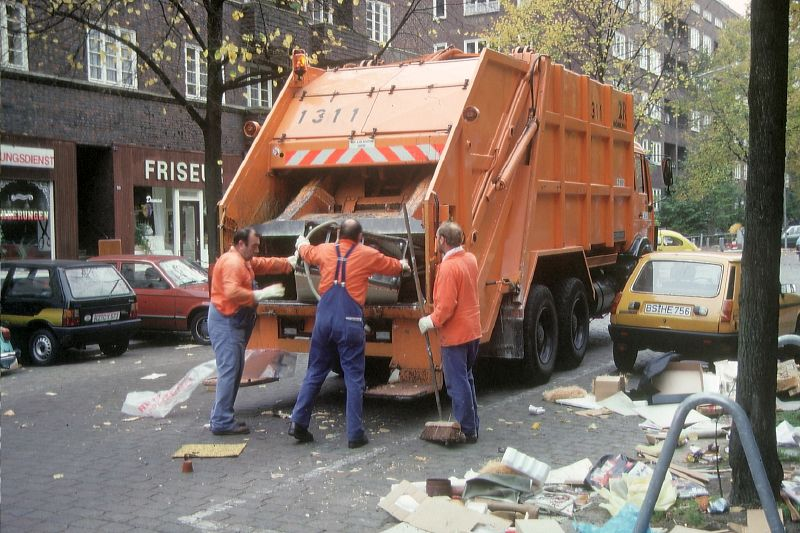
\includegraphics[scale=0.3]{img/garbage-collection.jpg}
   \end{center}
  \end{frame}
}

\ifbook{
  \mysubsubsection{"Garbage collection"}

  \paragraph{} Rapidement la gestion de la mémoire est devenu un tel frein au développement
  d'application, que de nombreuses recherches et expérimentations ont été entreprise pour construire
  une sorte de "méta application" qui assurerait la libération de la mémoire, simplifiant ainsi
  grandement la charge du développeur.

  \paragraph{} Ce \textbf{conteneur d'exécution\footnote{Le terme \textbf{conteneur d'exécution
  virtuelle} est une traduction somme toute très personnelle du terme anglais \textit{runtime
  container}. L'usage a imposé de désigne ce genre de container par leur nom (ex: JVM), plutôt que par
  un terme générique, comme système d'exploitation.}} se charge donc garder traces de toute
  allocations mémoires, mais aussi du nombre de référence vers ces dernières. Lorsque il n'existe
  plus, au sein, du programme, de référence vers un espace mémoire allouée, il ne reste plus qu'à
  faire le \textbf{nettoyage}. En anglais, on emploi fréquement le terme de \textit{\textbf{Garbage
  Collection}}.

  \mysubsubsubsection{Libération de la mémoire}

  \paragraph{} Comme toujours la création de ce nouveau \textbf{contexte d'exécution} a aussi été une
  opportunité d'introduire une nouvelle couche d'abstraction permettant au programme de se détacher du
  système d'exploitation.

  \paragraph{} Ainsi, on ne développe plus un programme à l'aide des primitives offertes par tel ou
  tel système d'exploitation, mais à l'aide de celles offertes par son conteneur d'exécution. Charge à
  ce conteneur de s'assurer du fonctionnement idoine de ces primitives quelques soit le système
  d'exploitation sur lequel il s'exécute.

  \mysubsubsection{Quelques conteneurs d'exécution}

  \paragraph{} La machine virtuelle Java est un exemple de tel conteneur d'exécution, mais aussi
  l'intépréteur python on PHP. Ces différents programmes exécutent un code, qu'il soit compilé ou non
  avant\footnote{C'est d'ailleurs cette seule notion de code compilé ou interprété qui distingue
  principalement la machine virtuelle Java des interpréteurs comme Python}, en abstrayant le système
  d'exploitation sous jacent.

  \begin{figure}[hb]
    \begin{center}
      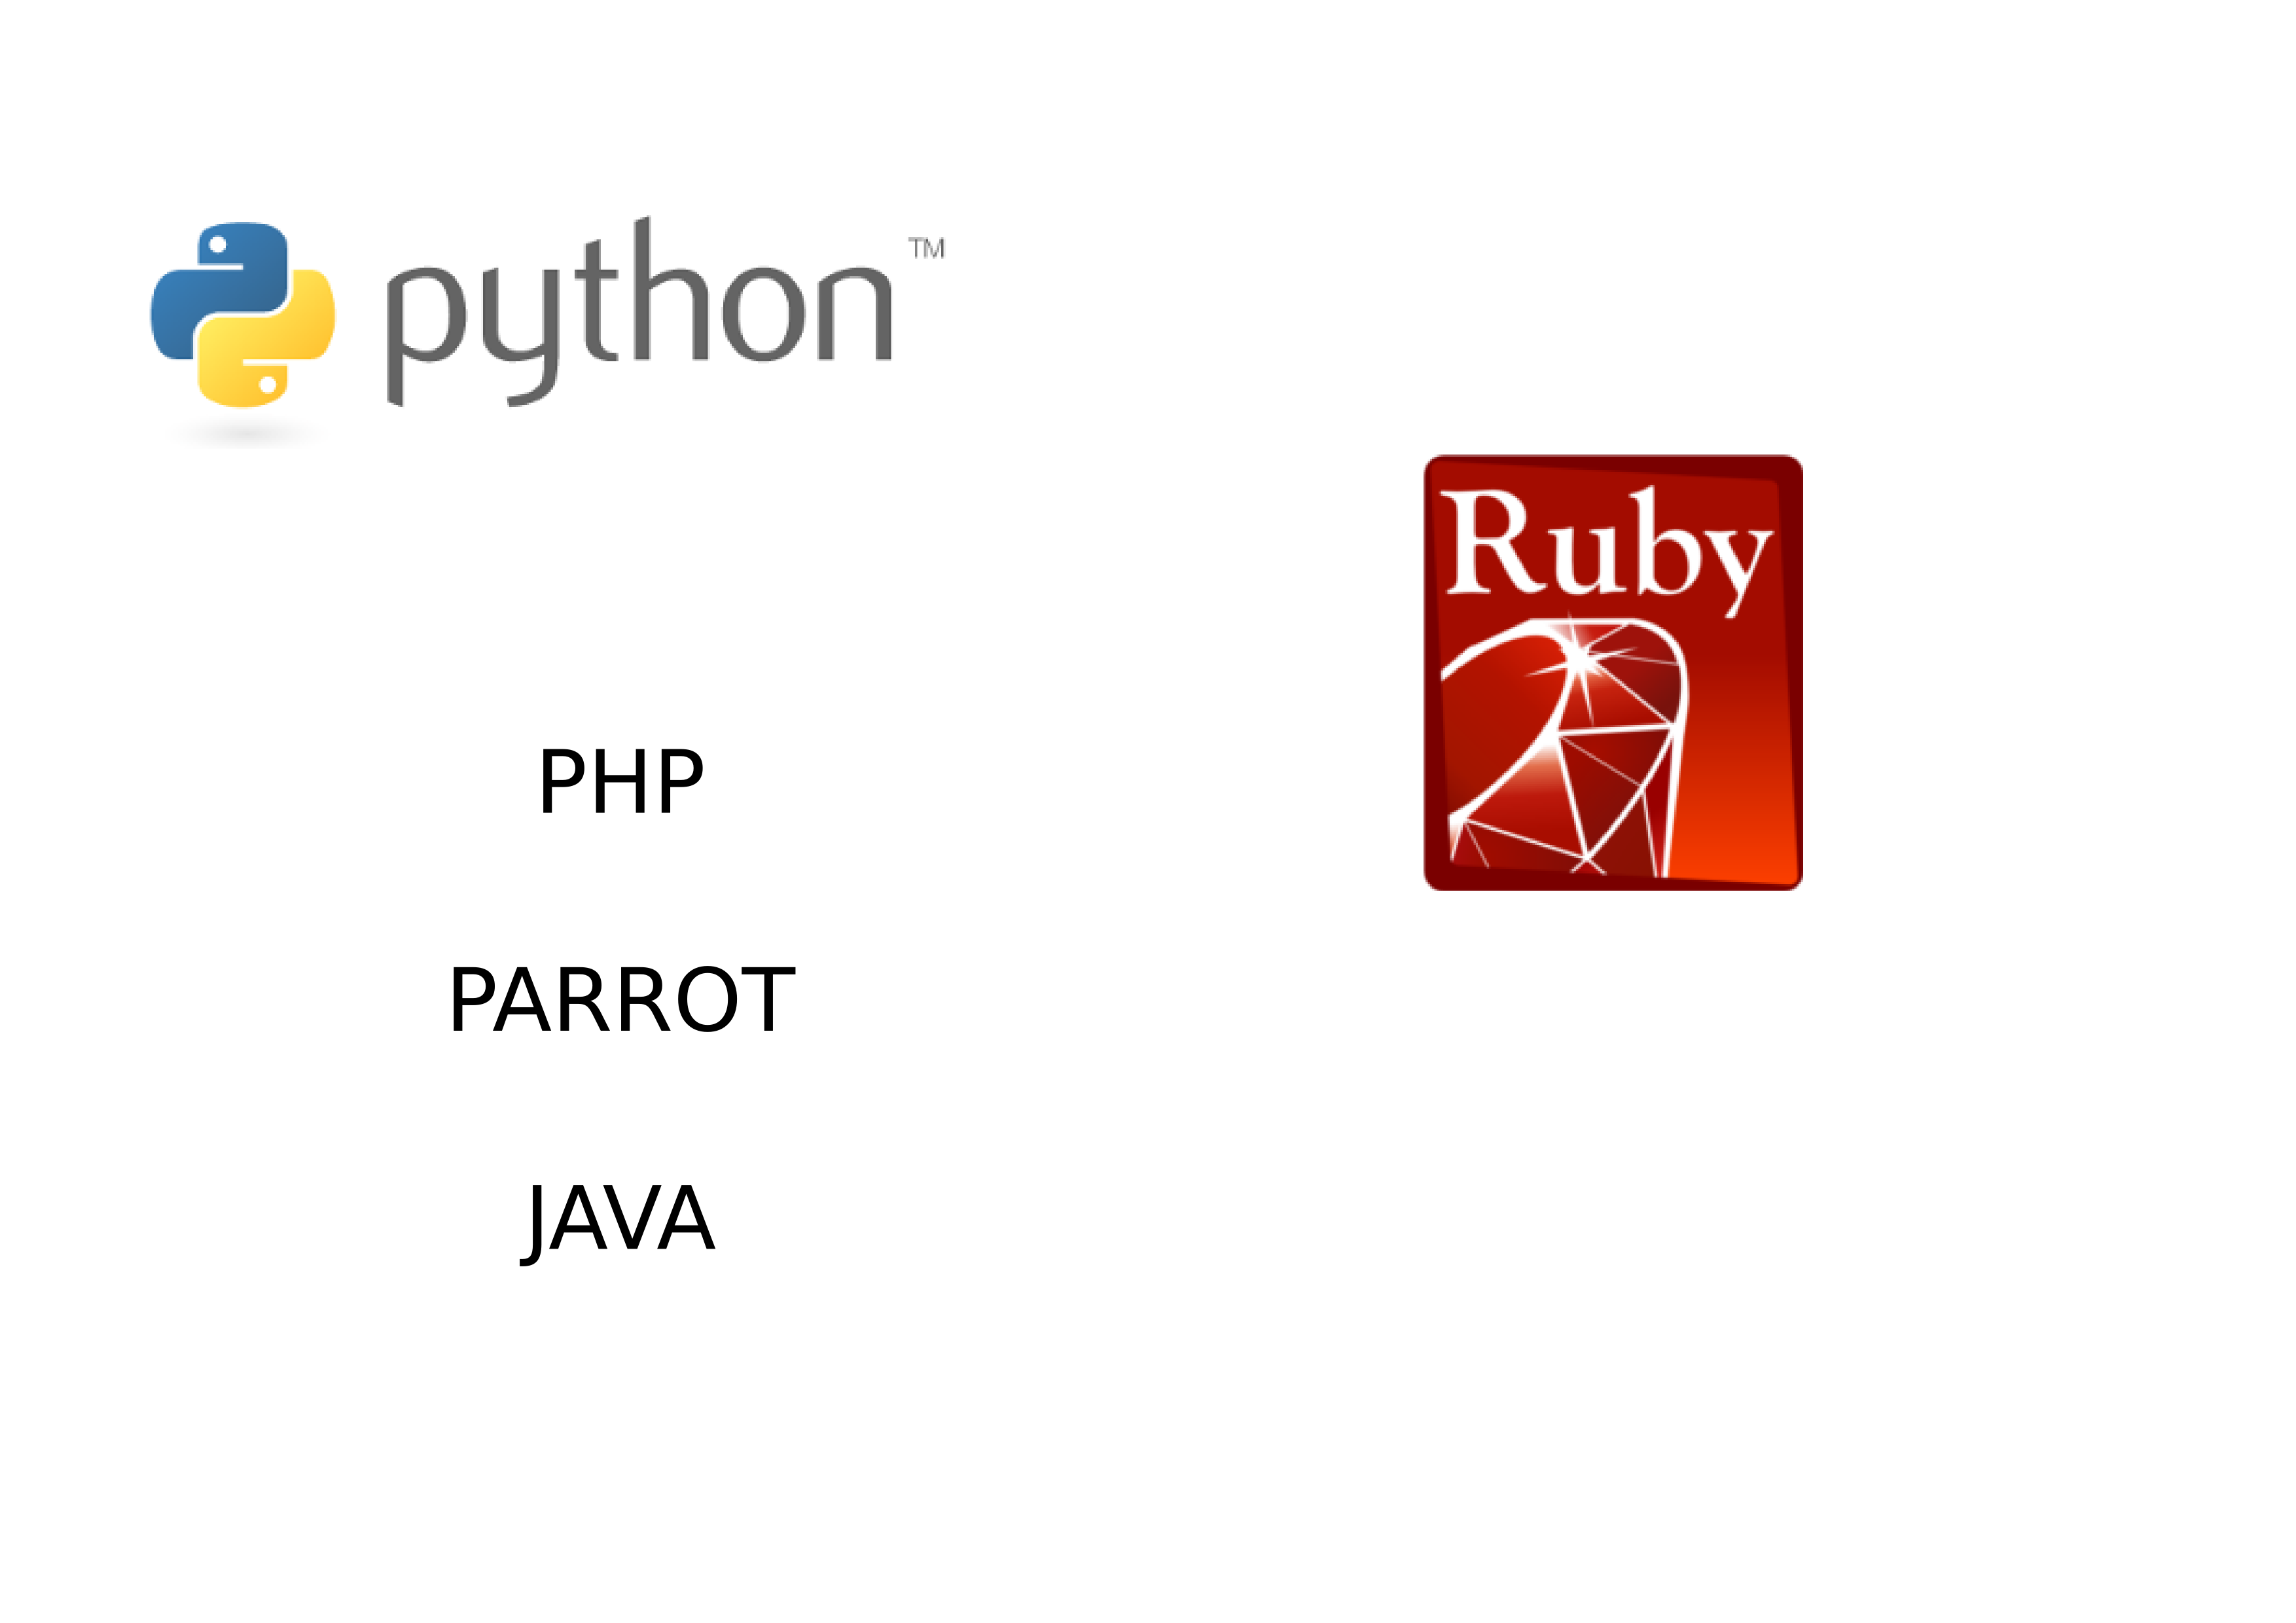
\includegraphics[scale=0.3]{img/sample-containers.png}
      \caption{Quelques conteneurs d'exécution le plus utilisé}
      \label{interop}
    \end{center}
  \end{figure}
}

\ifslide{
  \begin{frame}{Quelques conteneurs d'exécution}
   \begin{center}
     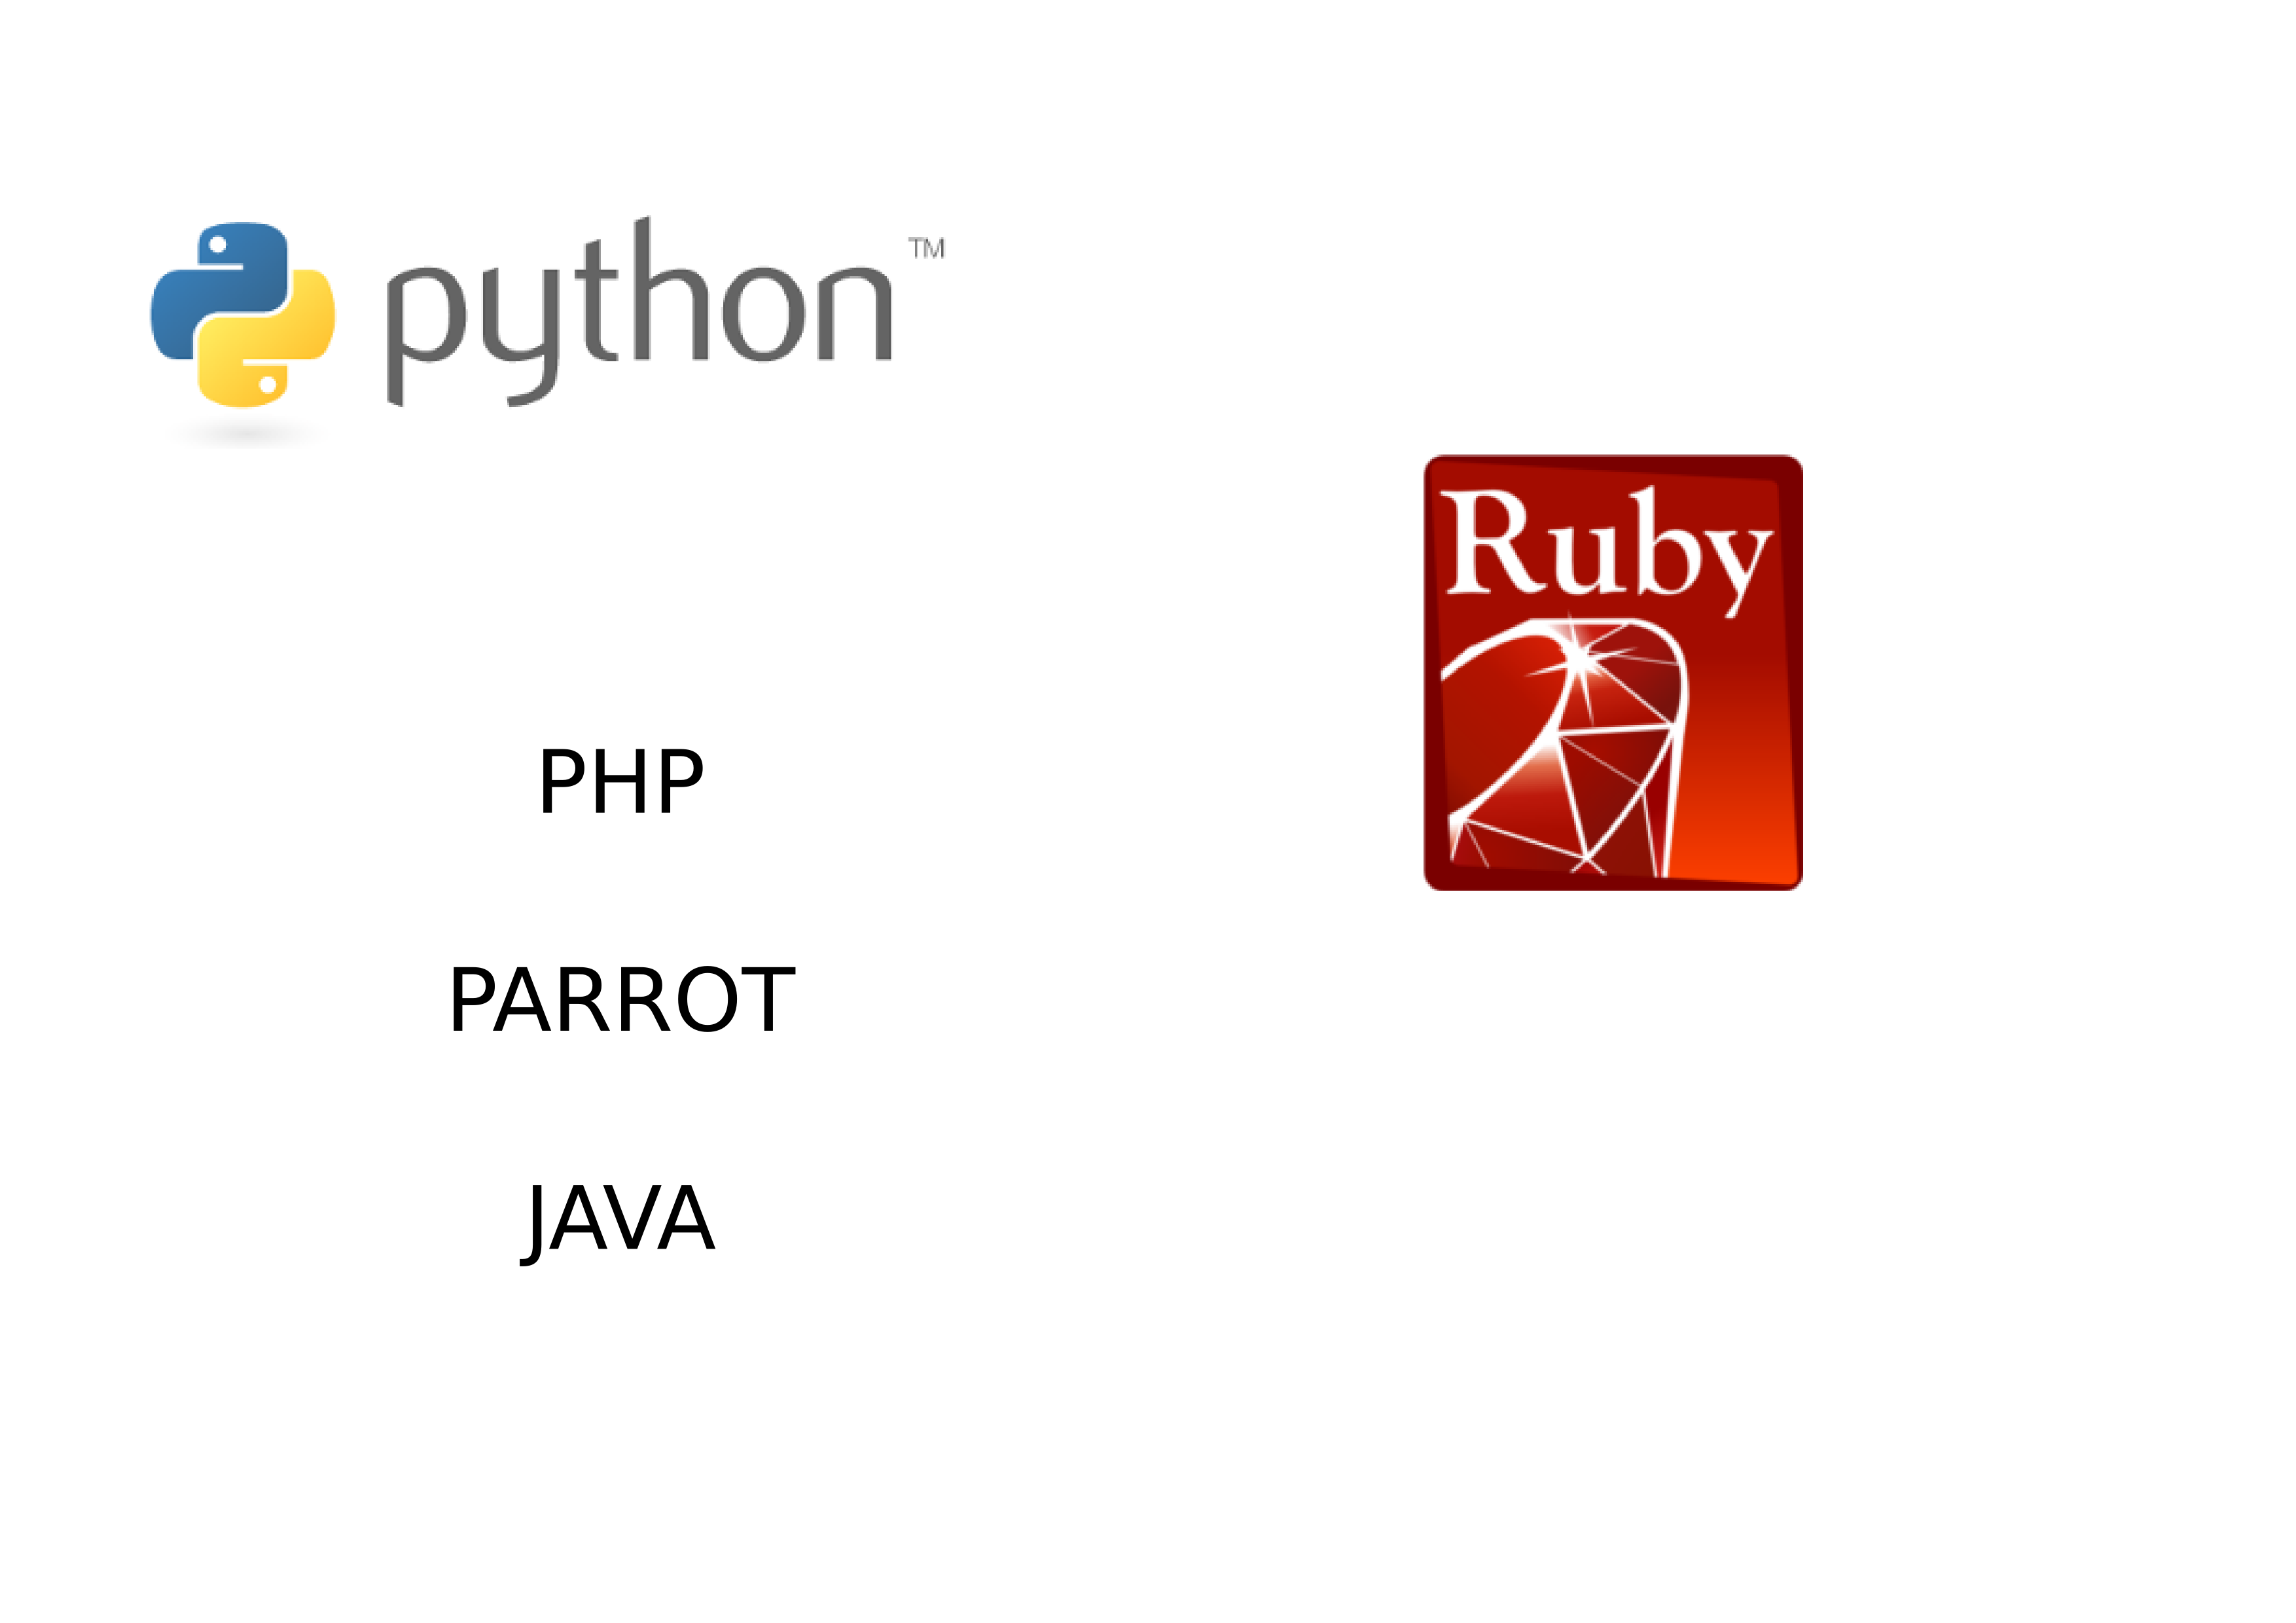
\includegraphics[scale=0.3]{img/sample-containers.png}
   \end{center}
  \end{frame}
}

\ifbook{
  \paragraph{} Si les conteneurs d'exécution abstrait le programe du système d'exploitation sur
  lequel il s'exécute, il est donc ainsi possible d'écrire un même programme Java ou un script
  Python de telle manière qu'il s'exécute de manière similaire sur différents système d'exploitation.

  \paragraph{} Il est donc ainsi possible d'écrire un même programme Java ou un script Python de telle
  manière qu'il s'exécute de manière similaire sur différents système d'exploitation. Attention
  néanmoins, il faut prendre soin de veiller à cette \textbf{interopérabilité} lors de la conception
  du programme, car l'on peut toujours aisément rendre son code très adhérant aux systèmes
  d'exploitation.

  \paragraph{} Attention néanmoins, si cette \textbf{interopérabilité} est rendue possible par
  l'utilisation d'un conteneur d'exécution, il faut néanmoins prendre soin de l'assurer lors de la
  conception du programme. En effet, on peut toujours aisément rendre son code très adhérant aux systèmes
  d'exploitation utilisé, et ceci malgré l'abstraction offerte par le conteneur.

  \paragraph{} Un exemple très concret de ce dernier point est l'utilisation de chemin de fichier
  spécifique à Windows©, plutôt que d'utiliser des URLs ou un chemin de fichier standard:

  \begin{figure}[hb]
    \begin{center}
      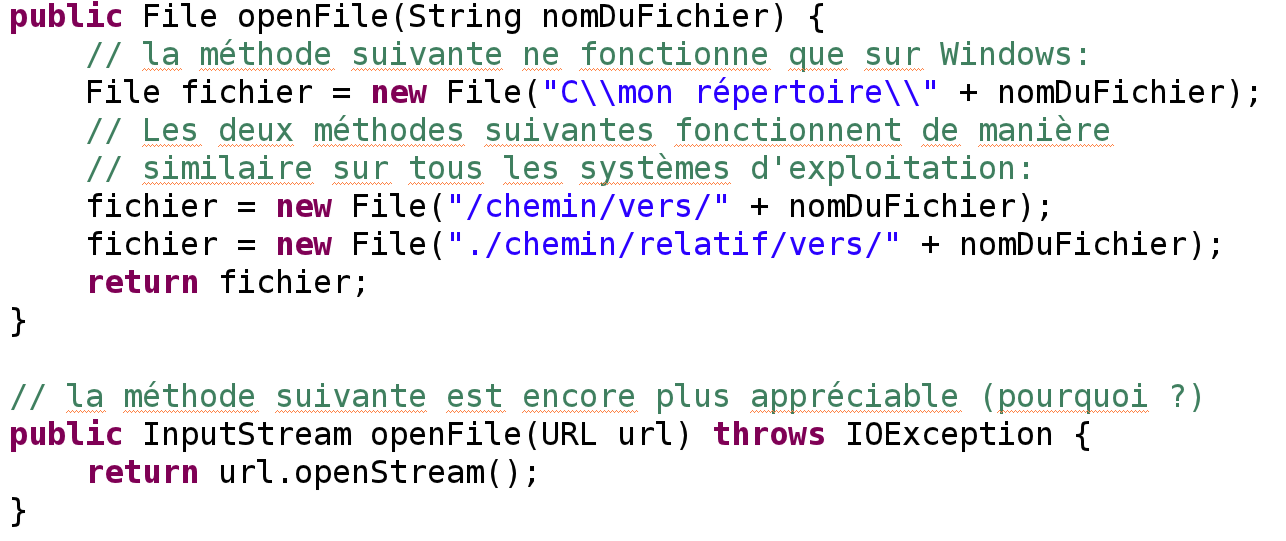
\includegraphics[scale=0.3]{img/interop.png}
      \caption{Exemple de problématique de portabilité au sein d'un conteneur}
      \label{interop}
    \end{center}
  \end{figure}
}

\ifslide{
  \begin{frame}{Interopérabilité}
   \begin{center}
     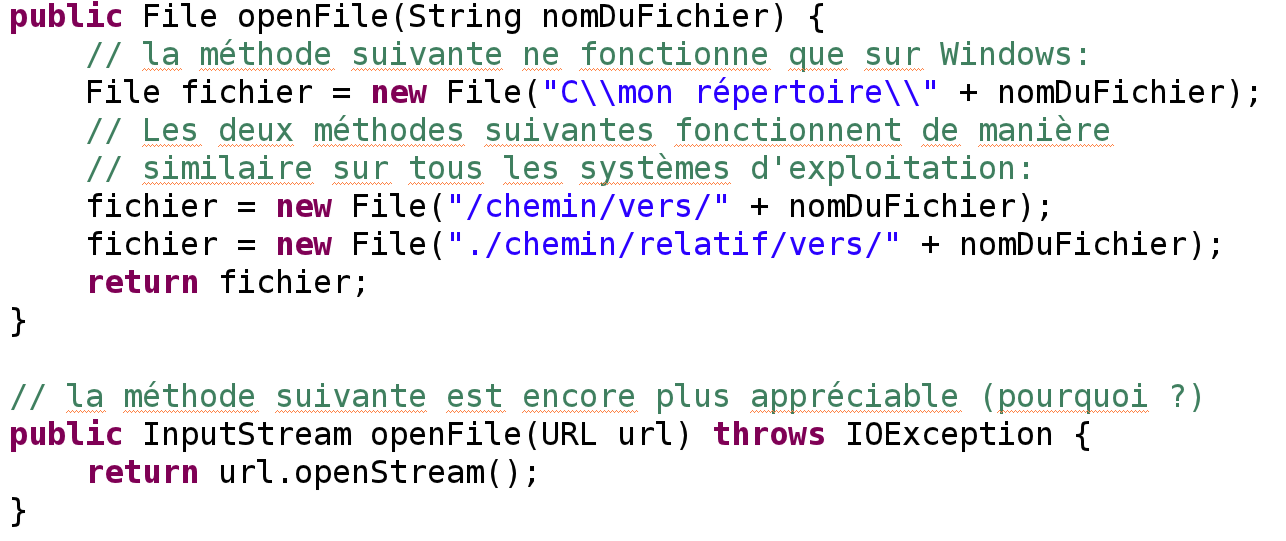
\includegraphics[scale=0.25]{img/interop.png}
   \end{center}
  \end{frame}
}

\ifbook{
  \paragraph{} C'est donc à propos des applications développées sur ces nouveaux conteneurs
  d'exécutions, et non plus de manière \textbf{native}, que nous allons désormais discuté. On
  notera, au passage, que, au bout du compte, ces conteneurs d'exécutions forment un premier
  \textbf{Middleware} pour l'application.
}

\mysubsection{Serveur d'applications}

\ifbook{

  \paragraph{} À l'aide des conteneurs précédemment évoqués, nous avons maintenant un cadre robuste et
  portable d'exécution de programme, nous offrant déjà des primitives relatives élaborés. Néanmoins,
  ces contextes d'exécutions sont toujours conçu pour exécuter un seul programme. Certes, ce programme
  peut créer des sous processus, mais en essence, le conteneur n'est pas conçu pour exécuter
  différentes applications de manière concurrente.

  \paragraph{} Nous allons voir apparaitre la notion de \textbf{serveur d'applications} - avec un 's'
  à applications, car l'enjeu est bien ici de pouvoir exécuter et \textbf{administrer} plusieurs
  application s'exécutant au sein d'un même et seule unique contexte d'exécution.

  \paragraph{} Voyons d'abord une définition du terme serveur d'application pour éclaircir un peu le
  sujet. La définition suivante est issue de \mylink{http://TODO/}{Wikipédia} (accédé le 21/12/2011):

  \paragraph{} \textit{Un serveur d'applications est un logiciel d'infrastructure offrant un contexte
  d'exécutiuon pour composants applicatifs. [...] Dans un sens strict les composants hébergés par le
  serveur d'applicatons ne sont pas de simples procédures ou scripts mais de réels composants
  logiciels conformes à un modèle de composants (EJB, COM, Fractal,...)}

  \paragraph{} Comme l'illustre assez bien la définition, ce serveur d'application, qu'il s'agisse
  d'un serveur d'application Java/JEE ou d'un serveur python tel que WebWare, est au final un
  \textbf{produit d'intégration}. En effet, ce serveur a aussi pour rôle de faciliter, pour les
  applications qu'il héberge, l'utilisation de programmes connexes, tel que les bases de données ou un
  serveur d'authenfication. Ainsi, le serveur d'applications permet l'intégration des applications à
  d'autres applications qui lui seront nécessaires.

  \paragraph{} Comme l'indique la définition, il est important de noter aussi qu'un serveur
  d'application abrite des \textbf{composants applicatifs}, et non de simple API. Le comportement de
  ces composants est ainsi beacoup plus configurable et ils offrent, pour la plupart, et à l'inverse
  des API, des mécanismes d'administration. En outre, les composants, là encore à l'inverse des APIs,
  sont plus "actifs". Nous reviendrons sur ce point tout au long du cours.

}

\ifbook {
  %TODO: definition d'un pool de connexion, intérêt...
  \mysubsubsection{Pool(s) de connexion}

  \paragraph{} Plutôt que de continuer de faire un résumé très théorique, et vraisemblablement peu
  pertinent sur ce sujet - qui ne ferait que satisfaire un goût très Mésopotamien de l'inventaire et
  des catalogues, nous allons voir un petit cas pratiques de configuration d'un pool de connexion.

  \paragraph{} Cette démarche sera, espérons-le, un peu moins aride, et devrait surtout permettre au
  lecteur de bien saisir les concepts sous jacents. Pour être didactique, cette section contiendra
  donc des extraits de codes et de configuration, mais là encore, l'objectif pédagogique ne sera pas
  retenir, ni même de forcément comprend l'intégralité de ces extraits, mais de bien cerner, de
  manière concrète, les concepts de plus haut niveau qui s'y rapportent.

  % TODO: RMI appli avec une connecion, qui dure 60s, renvoie une * toutes les 5s - barre de
  % progression - timeout, puis 2 utilisateurs concurrent
  % HTTP, RMI, AJP => offre pool de connexion, partagé entre les applications

  \mysubsubsection{Threads}
}

\ifslide{
  \demoframe{Threads}{
    \begin{block}{Configuration d'un "pool" de connexion}
      \begin{itemize}
        \item ToDo
      \end{itemize}
    \end{block}
  }
}

\ifbook{

  \paragraph{} De la même manière dont il existe un \textit{pool} de connexion, dont la gestion est
  confiée au serveur d'applications, la gestion du nombre de sous processus, ou plutôt de
  \textit{thread} pour reprendre le terme anglais plus souvent utilisé, est elle aussi confier au
  serveur d'application.

  \paragraph{} Dans une suite logique à ce que nous venons de voir, nous allons voir comment
  augmenter ou réduire le nombre de \textit{threads} qu'une application, s'exécutant au sein de
  JBoss, peut utiliser.

  \mysubsubsection{Première conclusion}

  \paragraph{} En étudiant, de manière sommaire, la gestion de types distincts de ressources (d'une
  part des connexions à une source de données, d'autres part le nombre de thread), nous pouvons
  désormais un peu mieux comprendre le rôle du serveur d'application.

  \paragraph{} Réel produit d'intégration, le serveur d'application prend donc en charge la gestion
  de nombreux, si ce n'est tous, aspects techniques, laissant les applications utilisées de simple
  API, standard pour la plupart. Une fois déployé au sein du serveur, on dispose néanmoins de
  nombreux mécanismes pour régler et configurer l'utilisation des ressources par l'application, de
  manière à exploiter au mieux possible ces dernières.

  \begin{figure}[hb]
    \begin{center}
      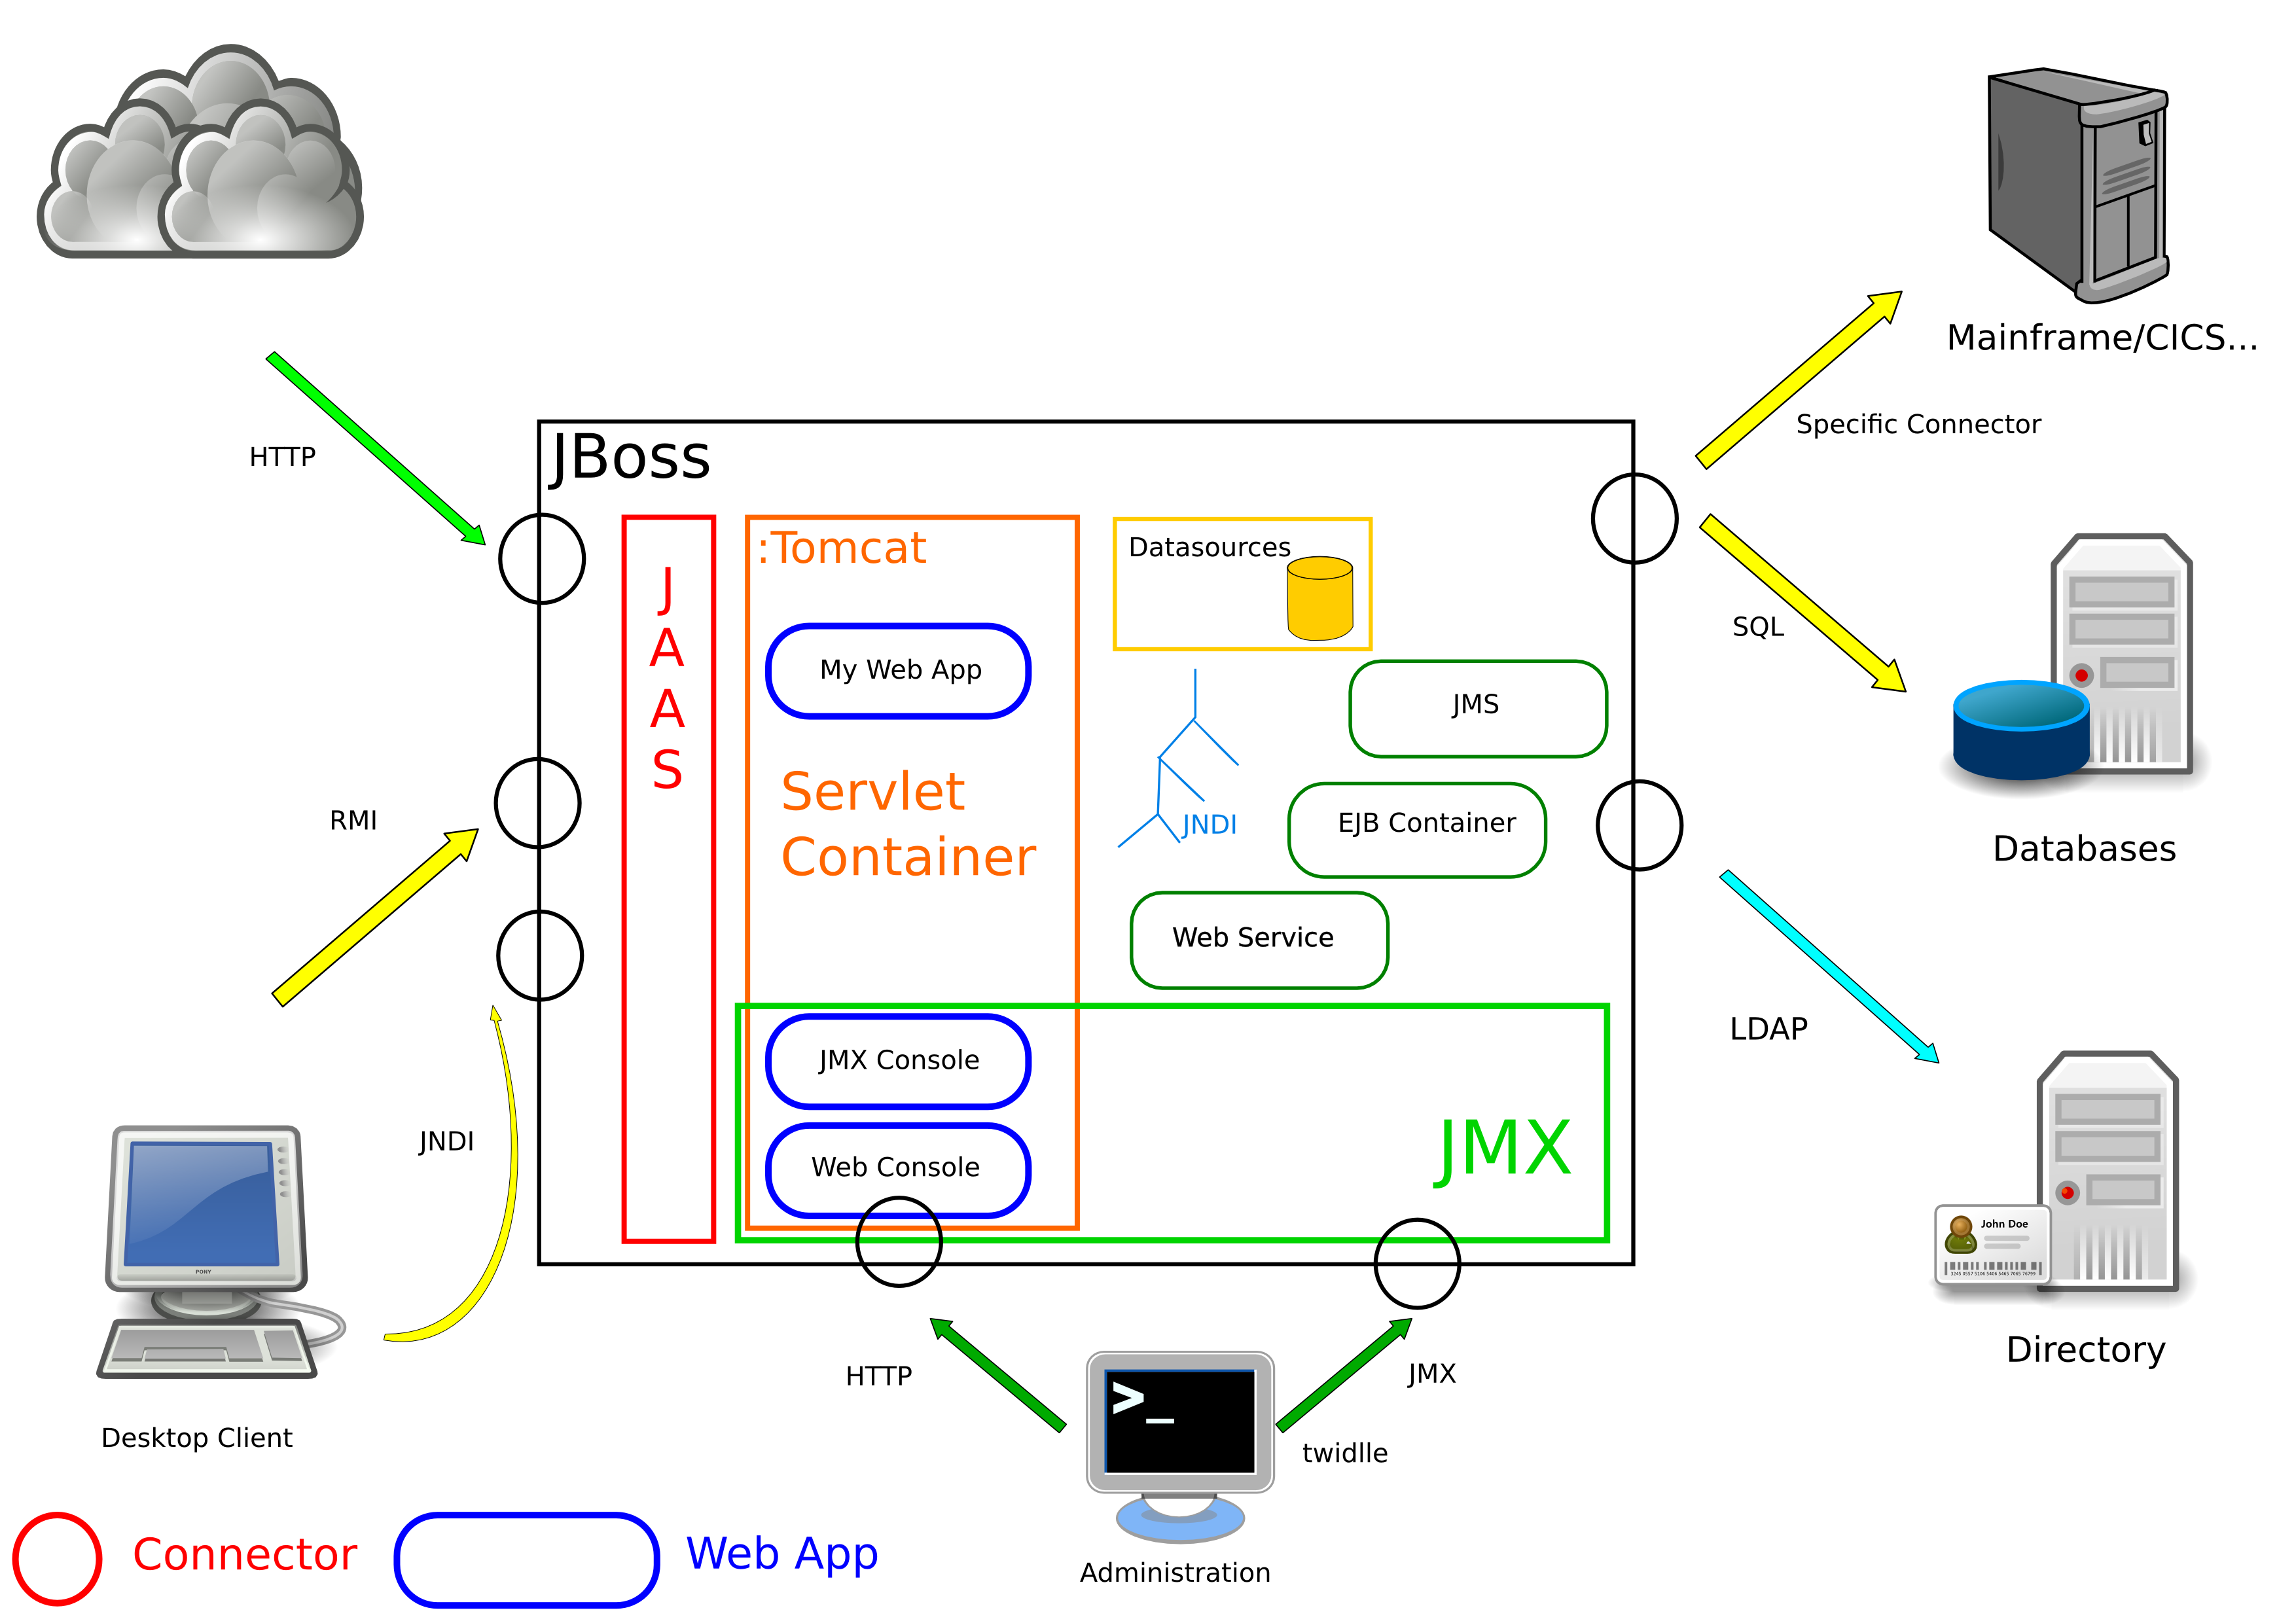
\includegraphics[scale=0.4]{img/integration-product.png}
      \caption{Exemple de serveur d'application: JBoss}
      \label{integration-product}
    \end{center}
  \end{figure}
}

\ifslide{
  \begin{frame}{Vision d'ensemble d'un serveur applicatif (JBoss AS)}
   \begin{center}
     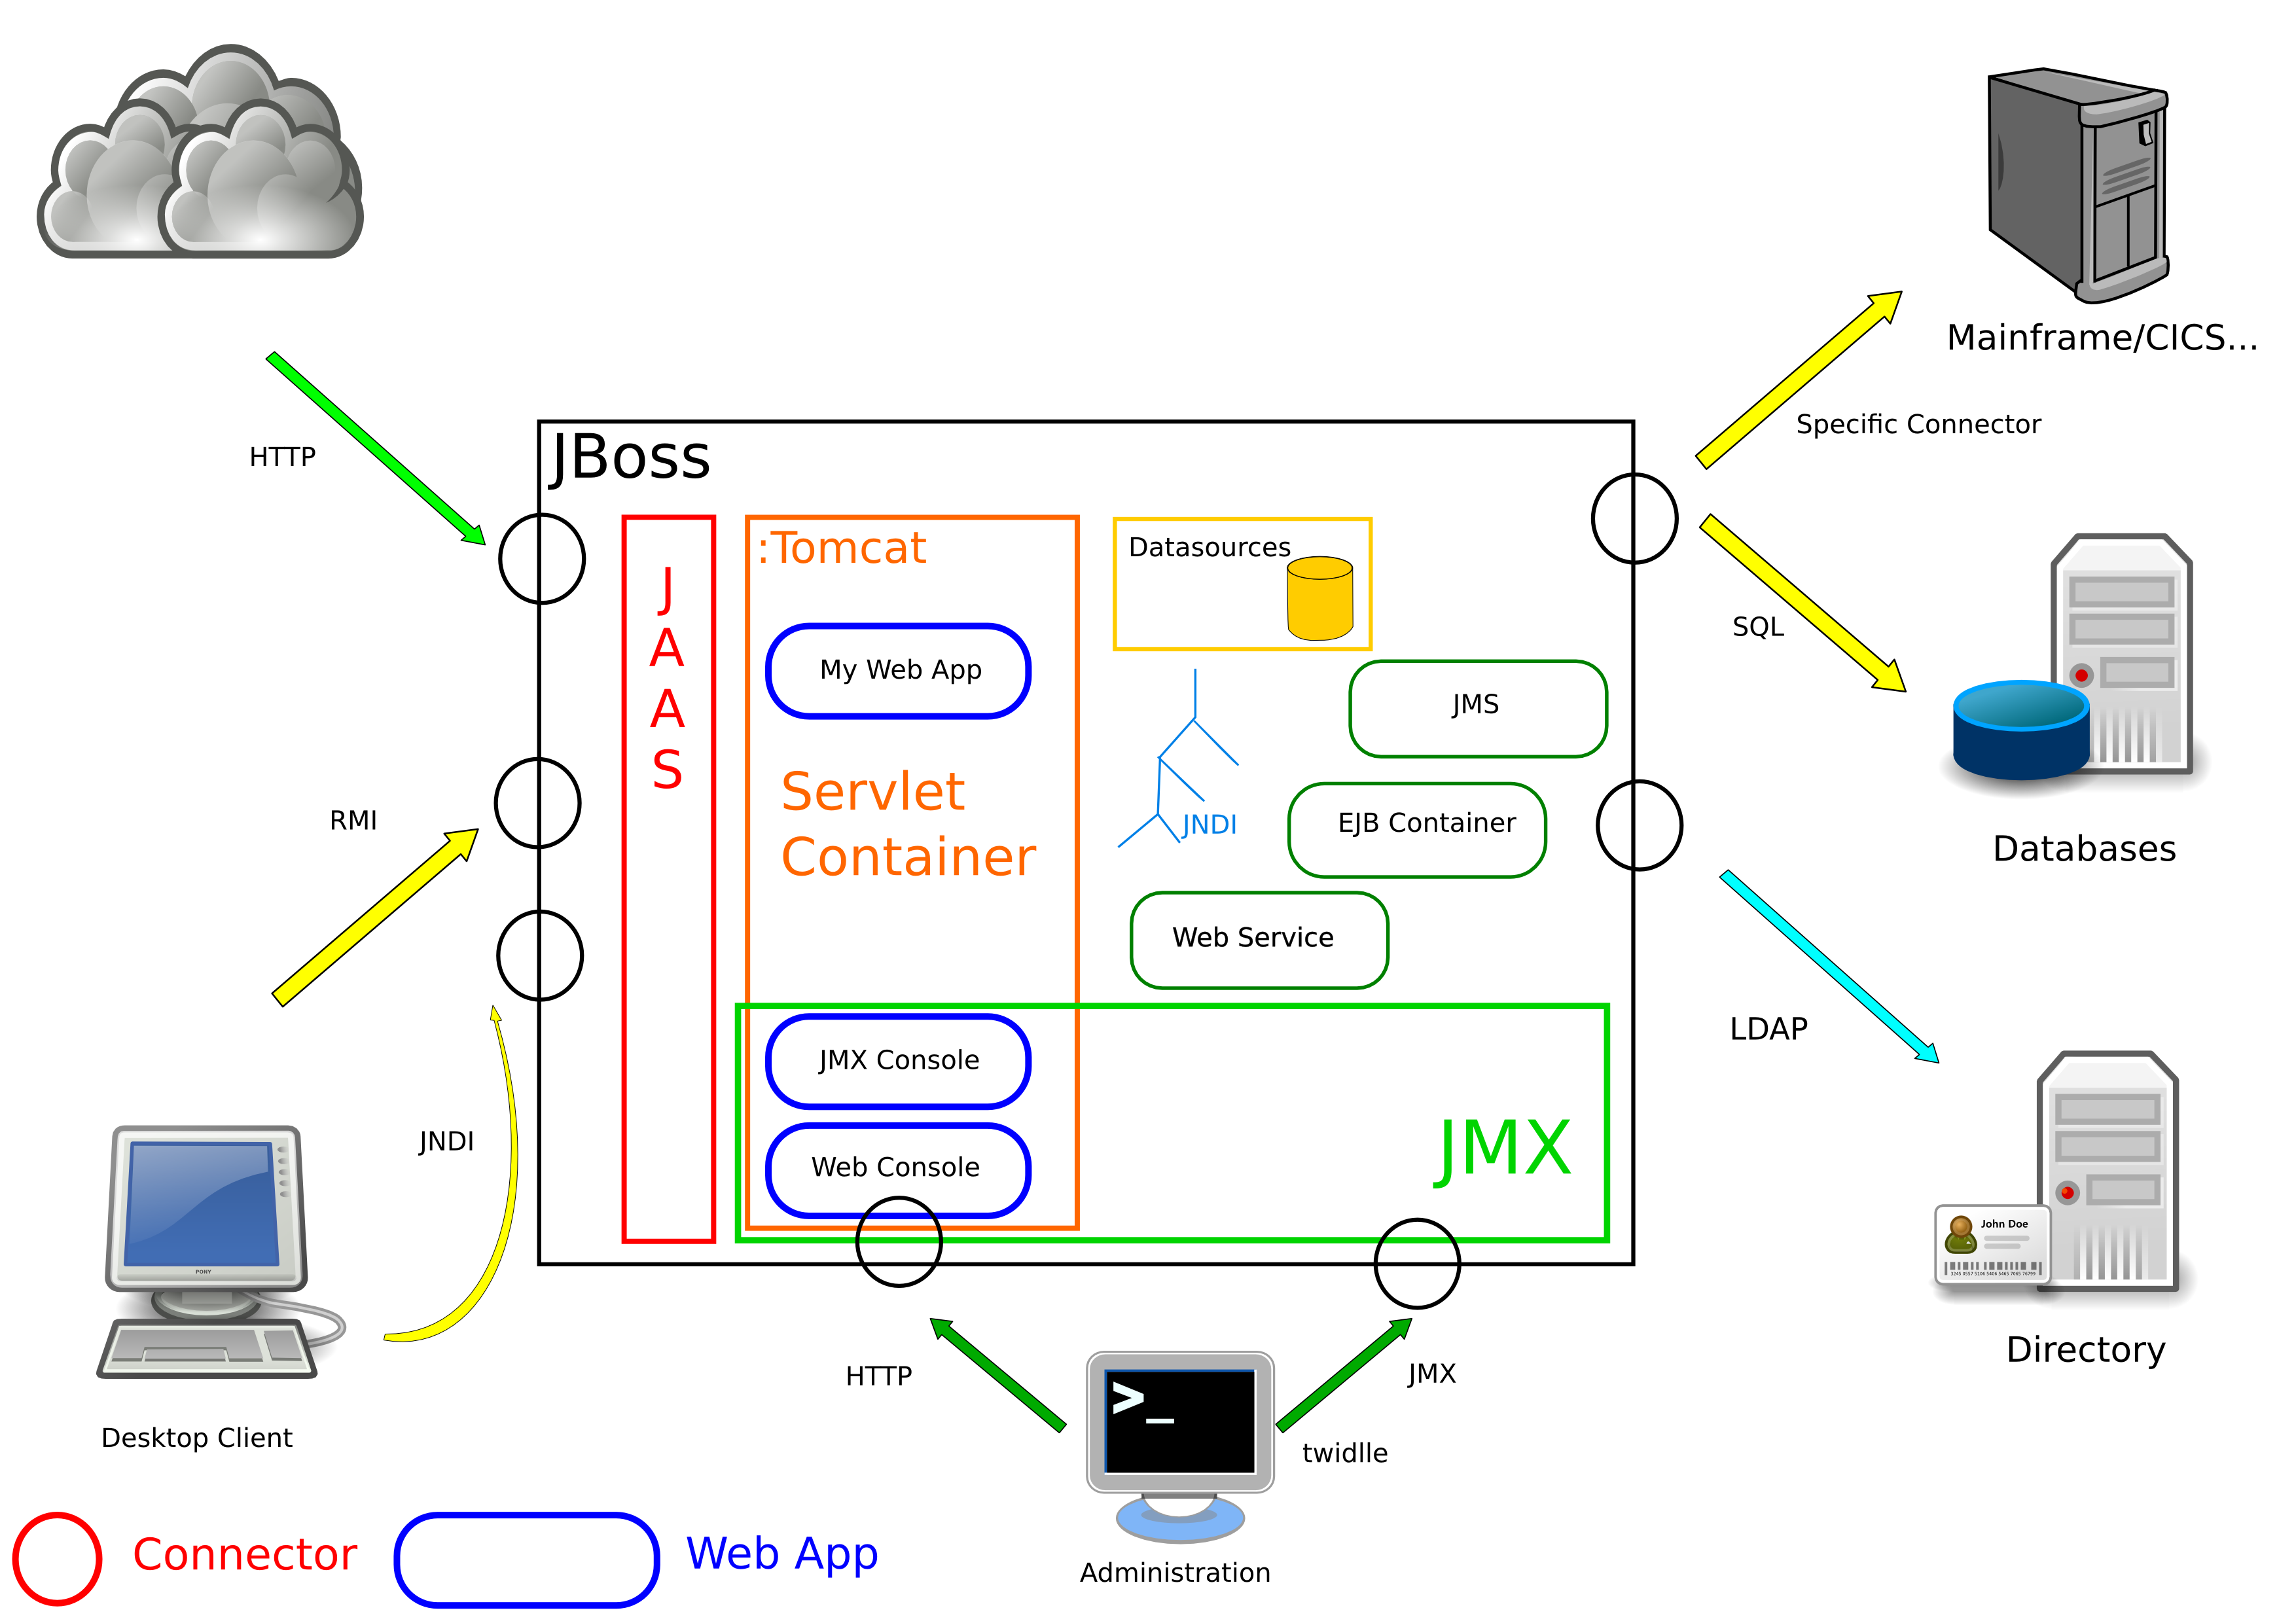
\includegraphics[scale=0.3]{img/integration-product.png}
   \end{center}
  \end{frame}
}
